%--------------------------------------------------------------------------
\chapter{}

%--------------------------------------------------------------------------
\section{The Mallalieu Property}
\label{mallalieu-section}

We now consider the $\T_n\M\I$ class of 12-tone rows with representative
\begin{equation}
	S = \{ 0, 1, 4, 2, 9, 5, 11, 3, 8, 10, 7, 6 \} \enspace.
\end{equation}
This series has the remarkable property that, if we include a dummy $13^\text{th}$ element, usually represented by an asterisk, then taking every $n^\text{th}$ element of $S$ produces a transposition of it, so that deriving transforms of a $S$ becomes a mechanical process.

\begin{example}
	Put $S^* = \{ 0, 1, 4, 2, 9, 5, 11, 3, 8, 10, 7, 6, * \}$. Then taking every zeroth order number of $S^* \mod 13$ yields trivially $S^*$ itself. Taking every first order number yields the row $\{ 1, 2, 5, 3, 10, 6, 0, 4, 9, 11, 8, 7, * \}$ which, upon removing the dummy symbol, becomes $\T_1(S)$. Repeating this procedure for every $n^\text{th}$ order number gives the sequence of $\T_i$-transforms of $S$ where the indices of transposition are totally-ordered, and correspond to the elements of $S$.
\end{example}

This most peculiar property, commonly known as the \emph{mallalieu} property, was first discovered by Pohlman Mallalieu \cite[285]{Lewin1966}. It is natural to ask at this point how many different 12-tone rows are there sharing this property. Unfortunately, there is only one such 12-tone row class under $\T_n\M\I$. We phrase below a little differently an argument given in \cite[17]{Morris1976}.

\begin{proposition}
	\cite[17]{Morris1976}
	\label{morris-mallalieu}
	A 12-tone row has the mallalieu property if and only if it is related by $\T_n\M\I$ to the row $S = \{ 0, 1, 4, 2, 9, 5, 11, 3, 8, 10, 7, 6 \}$.
	\begin{proof}
		One direction is just the straightforward check that every $\T_n\M\I$ transform of $S$ possesses the mallalieu property and is left to the reader. Conversely, if a row $R$ in its untransposed prime form has the mallalieu property, then there is a transposition that takes its order numbers in zeroth rotation, that is, the set $\{ 0, 1, 2, 3, 4, 5, 6, 7, 8, 9, 10, 11 \}$ to its order numbers in, say, first rotation, id est, the set $\{ 1, 3, 5, 7, 9, 11, 0, 2, 4, 6, 8, 10 \}$. We can write this transposition as a permutation $0 \mapsto 1, 1 \mapsto 3, 2 \mapsto 5, \cdots, 11 \mapsto 10 $, or in cycle notation as $\hat{\T}_k = ( 0 \; 1 \; 3 \; 7 \; 2 \; 5 \; 11 \; 10 \; 8 \; 4 \; 9 \; 6 )$. Note that $\hat{\T}_k$ is an operation on order numbers. Since $\hat{\T}_k$ corresponds to a transposition, there are only four candidates for $T_k$, its pitch-class domain counterpart, namely $k \in \{ 1, 5, 7, 11 \}$, because these are the only indices for which a transposition of pitch classes in cycle notation is a 12-cycle. Moreover, we do not need to consider the cases where $k \in \{5, 7, 11\}$, as $\T_5 = \M \circ \T_1$, $\T_7 = \M \I \circ \T_1$, and $\T_{11} = \I \circ \T_1$. Hence, without loss, we can set $k = 1$. But then $S$ is the only row in untransposed prime form where $\T_1$ induces the permutation $\hat{\T}_k$ from its order numbers in zeroth rotation to its order numbers in first rotation. To see that, one needs to equate the cycles of $\hat{\T}_k$ with those of $\T_1$.
	\end{proof}
\end{proposition}

A way of looking at the mallalieu property from the standpoint of replacing, for any 12-tone row, its order-number row by the array of integers $\{ 1, 2, 3, 4, 5, 6, 7, 8, 9, 10, 11, 12 \}$ modulo 13 is provided in \cite[278]{Lewin1966}. It is easy to see that such an array has the same structure as the array $S^*$ constructed above, if we consider multiplication as the group operation. This is easily seen to be an isomorphism between the integers modulo 12 and the group of units modulo 13. One of the advantages of this approach is that we can dispense with the extra symbol altogether, and just use the indices from 1 to $p - 1$. We shall, however, still refer to the row of order numbers as $S^*$, the context making it clear whether we are constructing it with an asterisk or not. The process of taking every $n^\text{th}$ element of a 12-tone row becomes then just the aforementioned multiplicative group operation on order numbers, that is, multiplying order numbers by $k \pmod{13}$ is the same as taking every $k^\text{th}$ element of a row.

\begin{example}
	Let $S = \{ 0, 1, 2, 3, 4, 5, 6, 7, 8, 9, 10, 11 \}$ and $S^*$ be as above. Then $\M_3(S^*) = \{ 3, 6, 9, 12, 2, 5, 8, 11, 1, 4, 7, 10 \}$, which corresponds to the row $V = \{ 2, 5, 8, 11, 1, 4, 7, 10, 0, 3, 6, 9 \}$. The row $V$ can be equivalently constructed by placing an asterisk at the $13^\text{th}$ order number of $S$, then taking every third element. However being able to express the process through multiplication, rather than mechanically, greatly facilitates its theoretical description, as well as any algorithmic implementation thereof. The fact that $V$ and $S$ are not related by $\T_n\M\I$ reflects the fact that neither $S$ nor $V$ have the mallalieu property.
\end{example}

It should be of interest to many composers whether other $n$-TET systems are capable of producing mallalieu rows, and if so, how many. Unfortunately, answering this question is not as straightforward as the above discussion, since we cannot in general rely on the isomorphism that constitutes the proof of \ref{lewin-mallalieu}. Whenever we can, however, the existence of mallalieu rows is easily verified.

\begin{proposition}
	\label{lewin-mallalieu}
	\cite[285]{Lewin1966}
	For $p$ a prime, every $(p - 1)$-TET system is capable of producing a mallalieu row.
	\begin{proof}
		For every prime $p$, the group of units modulo $p$ is isomorphic to $\mathbb{Z} / (p - 1) \mathbb{Z}$. The mallalieu property in these cases can be seen as the aforementioned isomorphism, where $\mathbb{Z} / (p - 1) \mathbb{Z}$ is the group of transpositions of a row, and $(\mathbb{Z} / p \mathbb{Z})^\times$ is its multiplicative group on order numbers. The number of mallalieu rows in each $(p - 1)$-TET system is then the number of isomorphisms $\mathbb{Z} / (p - 1) \mathbb{Z} \to (\mathbb{Z} / p \mathbb{Z})^\times$, that is, the order of the group of automorphisms of $\mathbb{Z} / (p - 1) \mathbb{Z}$. Since for every prime $p$ we have $|\Aut(\mathbb{Z} / (p - 1) \mathbb{Z})| \geq 1$, every $(p - 1)$-TET system is capable of producing a mallalieu row, as desired.
	\end{proof}
\end{proposition}

In face of \ref{lewin-mallalieu}, \ref{morris-mallalieu} becomes just the special case where $p = 13$, as demonstrated in the next example.

\begin{example}
	\cite[8]{Lewin1976a}
	\cite[9]{Babbitt1976}
	The number of isomorphisms $\mathbb{Z} / 12 \mathbb{Z} \to (\mathbb{Z} / 13 \mathbb{Z})^\times$ is equal to
	\begin{equation}
		|\Aut\big((\mathbb{Z} / 12 \mathbb{Z})^\times\big)| = 4 \enspace.
	\end{equation}
	We can construct these isomorphisms by mapping a generator of $\mathbb{Z} / 12 \mathbb{Z}$, say $\bar{1}$, to the generators of $(\mathbb{Z} / 13 \mathbb{Z})^\times$, namely $\bar{2}, \bar{6}, \bar{7}$ and $\overline{11}$. Explicitly, we get the four maps $i \pmod{12} \mapsto 2^i \pmod{13}$, $i \pmod{12} \mapsto 6^i \pmod{13}$, $i \pmod{12} \mapsto 7^i \pmod{13}$, and $i \pmod{12} \mapsto 11^i \pmod{13}$. We leave the verification that these maps are well defined and bijective to the reader. Denote the first map by $\varphi$. Then
	\begin{equation}
		\varphi(a + b) = 2^{a + b} = 2^a \cdot 2^b = \varphi(a) \cdot \varphi(b) \enspace,
	\end{equation}
	so $\varphi$ is an isomorphism. The verification that the other three maps are isomorphisms is identical. Define $\varphi^{-1} : (\mathbb{Z} / 13 \mathbb{Z})^\times \to \mathbb{Z} / 12 \mathbb{Z}$ by $\varphi^{-1}(\log i \pmod{13}) = i \pmod{12}$. Then $\varphi^{-1}$ is easily seen to be the inverse of $\varphi$. Let $S^* = \{ 1, 2, \dots, 11, 12 \}$ be a series of order numbers written multiplicatively. Then
	\begin{equation}
		\varphi^{-1}(S^*) = \{ \log 1, \log 2, \dots, \log 12 \} \pmod{13} =
		\{ 0, 1, 4, \dots, 7, 6 \} \enspace,
	\end{equation}
	which by \ref{morris-mallalieu} is one of the untransposed 12-tone rows that have the mallalieu property.
\end{example}

We conclude this section by exposing some well-known isomorphisms between groups of pitch-class operations and abstract groups.

\begin{proposition}
	\cite[127]{FripertingerLackner2015}
	We have the following isomorphisms:
	\begin{gather}
		\langle \T \rangle \cong C_{12} \\
		\langle \T, \I \rangle \cong D_{24} \\
		\langle \I, \R \rangle \cong V_4 \\
		\langle \T, \I, \R \rangle \cong D_{24} \oplus \mathbb{F}_2 \\
		\langle \T, \I, \M \rangle \cong \Aff_1(C_{12}) \\
		\langle \T, \I, \M, \R \rangle \cong \Aff_1(C_{12}) \oplus \mathbb{F}_2
	\end{gather}
\end{proposition}

\begin{example}
	\cite[207]{Starr1984}
	\label{starr-webern-example}
	This examples provides a strategy to unravel the basic total order in Webern's Op.~27. It is somewhat paradoxical in the sense that unveiling the row requires prior knowledge of it. Consider the opening bars in Webern's Op.~27 depicted in Fig.~\ref{fig:webern-27}, as well as their aggregate realization given in Fig.~\ref{fig:webern-aggregate}.

    \begin{figure}[htbp]
    	\centering
		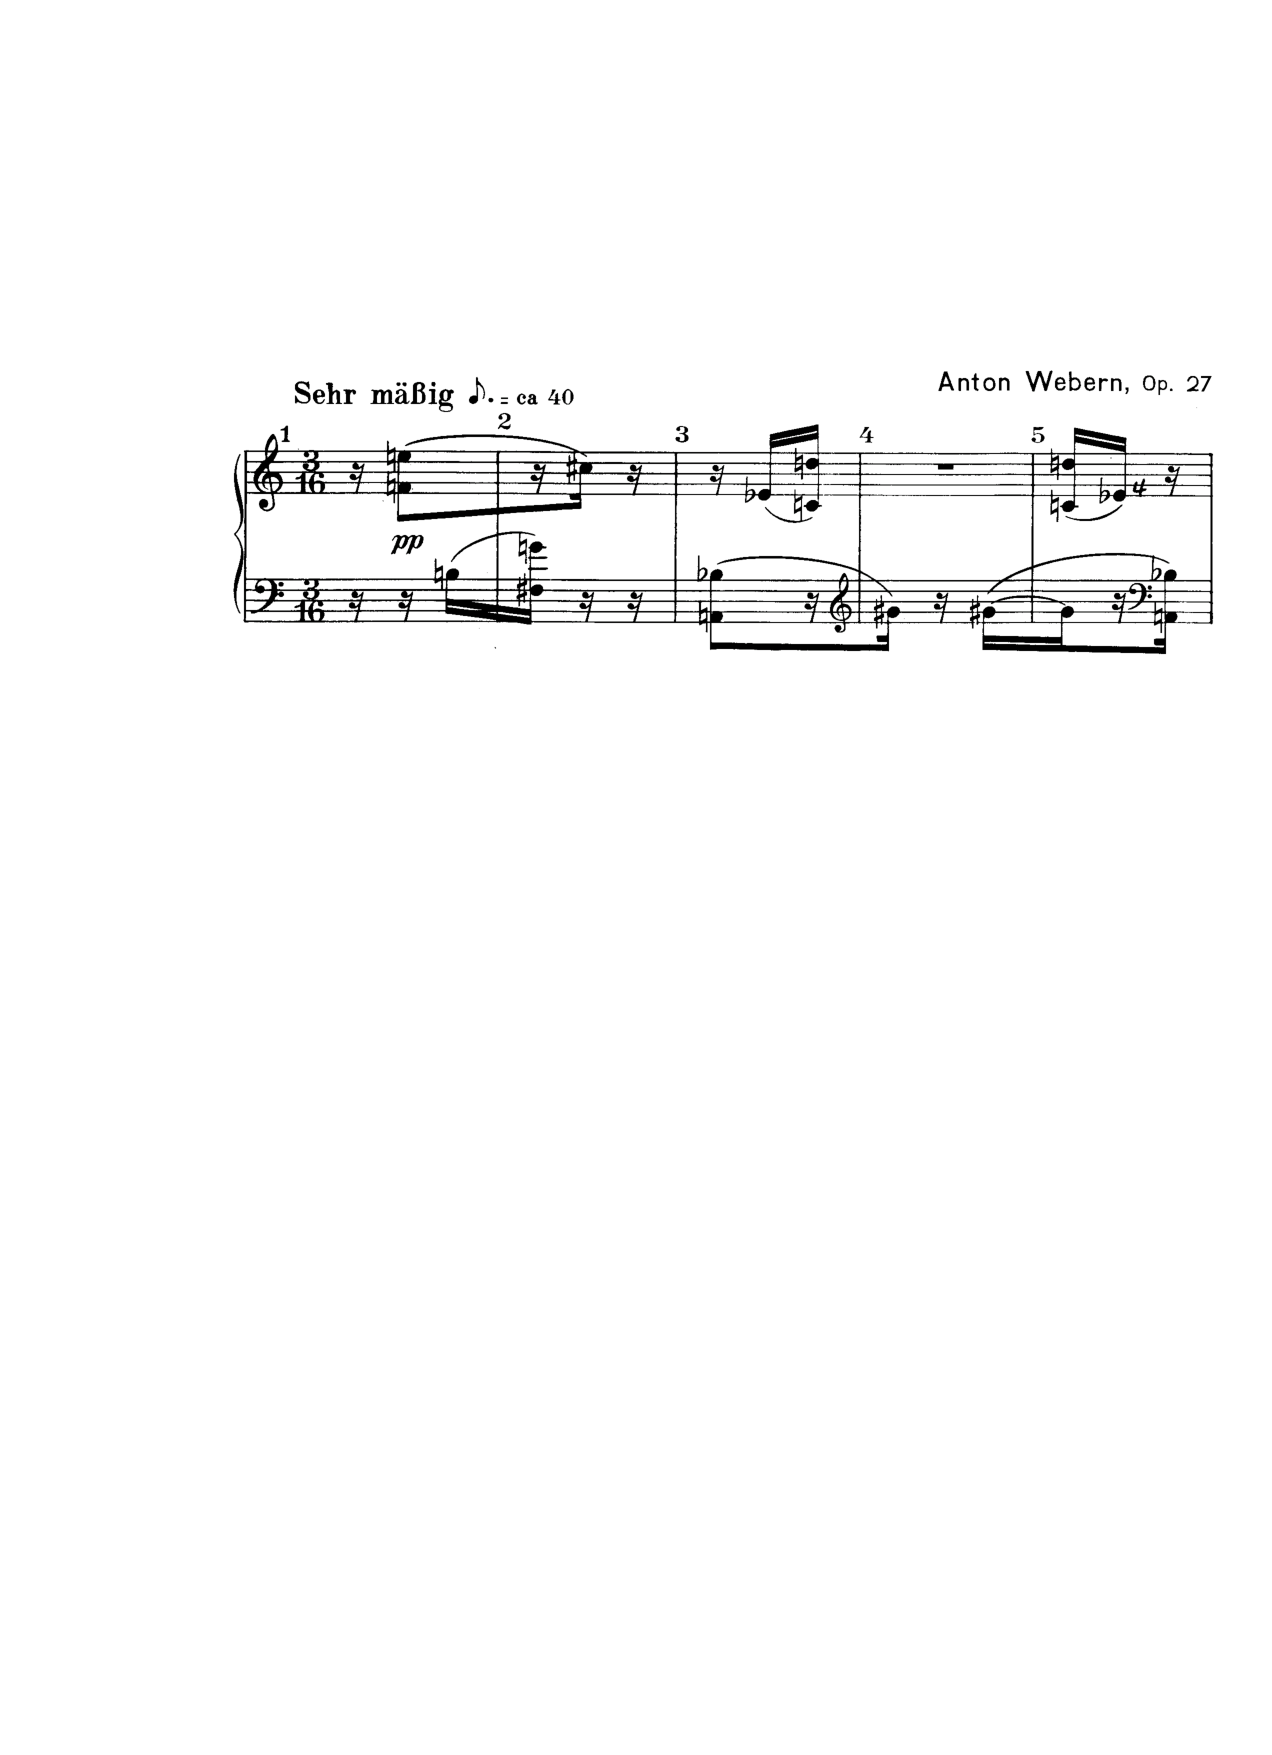
\includegraphics[width=6.5in]{figures/webern1.pdf}
		\caption[Bars 1--7 in Webern's Op.~27]{The initial bars in Webern's Op.~27.}
    	\label{fig:webern-27}
	\end{figure}

    \begin{figure}[htbp]
    	\centering
		\begin{tikzcd}
        	& E \arrow[dr] && G \arrow[dr] && B\flat \arrow[dr] && D \arrow[dr] & \\
        	* \arrow[dr] \arrow[ur] && B \arrow[dr] \arrow[ur] && C\sharp \arrow[dr] \arrow[ur] && E\flat \arrow[dr] \arrow[ur] && G\sharp \\
        	& F \arrow[ur] && F\sharp \arrow[ur] && A \arrow[ur] && C \arrow[ur] &
    	\end{tikzcd}
		\caption[Aggregate Realization of Bars 1--7 in Webern's Op.~27]{An aggregate realization of the initial bars in Webern's Op.~27. At its very first presentation, the total order used to generate the piece cannot be discerned. Moreover, the partial order that can actually be heard intercalates the total order's two hexachords, a procedure that can be construed as a form of derivation.}
    	\label{fig:webern-aggregate}
	\end{figure}

	\noindent Instead of the aggregate realization in Fig.~\ref{fig:webern-aggregate}, however, the fact that the basic series is known to be $S = \{ 4, 5, 1, 3, 0, 2, 8, 9, 10, 6, 7, 11 \}$ is used take the initial bars seen in Fig.~\ref{fig:webern-27}, and rewrite an aggregate realization, call it $D_1$, of them as in Fig.~\ref{fig:webern-aggregate-b}.

	\begin{figure}[htbp]
    	\centering
		\begin{tikzcd}
	    	& [-1em] E \arrow[dr] & [-1em] & [-1em] & [-1em] D \arrow[rd] & [-1em] & [-1em] B\flat \arrow[dr] & [-1em] & [-1em] G \arrow[dr] & [-1em] \\
	    	* \arrow[dr] \arrow[ur] & [-1em] & [-1em] C\sharp \arrow[r] & [-1em] E\flat \arrow[dr] \arrow[ur] & [-1em] & [-1em] G\sharp \arrow[dr] \arrow[ur] & [-1em] & [-1em] * \arrow[dr] \arrow[ur] & [-1em] & [-1em] B \\
	    	& [-1em] F \arrow[ur] & [-1em] & [-1em] & [-1em] C \arrow[ur] & [-1em] & [-1em] A \arrow[ur] & [-1em] & [-1em] F\sharp \arrow[ur] & [-1em]
    	\end{tikzcd}
    	\caption[Another Aggregate Realization of Bars 1--7 in Webern's Op.~27]{The underlying partial order depicted in this aggregate realization is denoted by $D_1$.}
    	\label{fig:webern-aggregate-b}
	\end{figure}

	\noindent It is not too far-fetched to assume such an analysis. Whereas Fig.~\ref{fig:webern-aggregate} represented a first-time hearing depiction of bars 1--7, Fig.~\ref{fig:webern-aggregate-b} can be achieved by, say, a performer who realizes the voice-crossing of the series along its reflection axis. Having come to this conclusion, parsing bars 8--10 becomes a bit less daunting. Fig.~\ref{fig:webern-27-b} shows bars 8--10 in Op.~27, and Fig.~\ref{fig:webern-aggregate-c} is a normalized aggregate realization of the passage. Normalized here means that the series being displayed in the music is $\T_{10}\I(S) = \{ 6, 5, 9, 7, 10, 8, 2, 1, 0, 4, 3, 11 \}$, but instead the aggregate realization is set to $S$, in order to facilitate taking intersections of both partial orders later. $\T_{10}\I(S)$ begins with the right hand in bar 8, moves to the left hand in bar 9, and the very last note (which is not showing) is a high B the right hand again has in bar 11. At this point, any confidence that a series can be heard by the listener is severely damaged. It is unlikely that the average performer will have obtained, or even cared to obtain, a good grasp on what the series really is.

	\begin{figure}[htbp]
    	\centering
		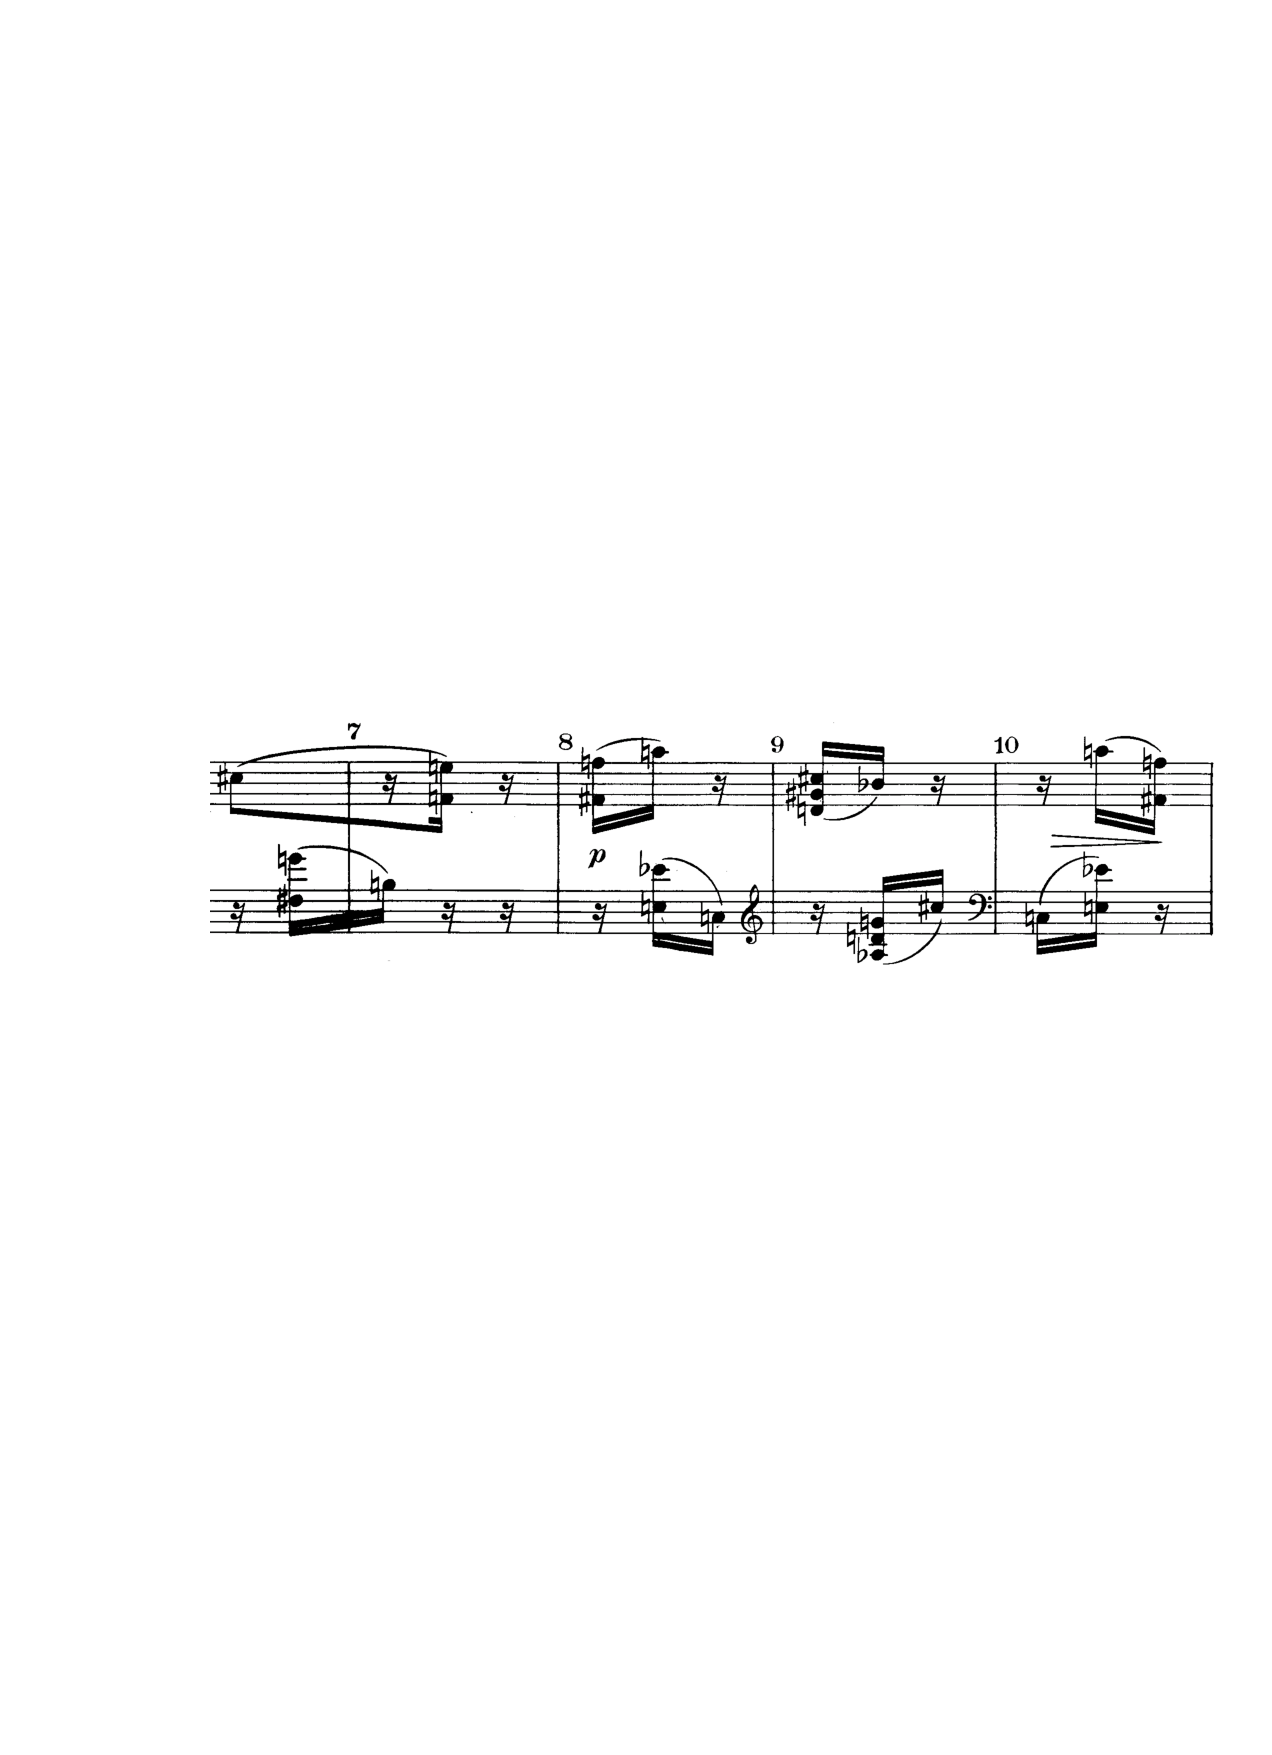
\includegraphics[width=6.5in]{figures/webern2.pdf}
		\caption[Bars 8--10 in Webern's Op.~27]{Bars 8--10 in Webern's Op.~27.}
    	\label{fig:webern-27-b}
	\end{figure}

	\begin{figure}[htbp]
    	\centering
		\begin{tikzcd}
	    	&&& E\flat \arrow[ddr] &&&& \\
	    	& E \arrow[dr] && D \arrow[dr] &&& G \arrow[dr] & \\
	    	* \arrow[ur] \arrow[dr] && C\sharp \arrow[ur] \arrow[dr] \arrow[uur] \arrow[ddr] && A \arrow[r] & B\flat \arrow[ur] \arrow[dr] && B \\
	    	& F \arrow[ur] && C \arrow[ur] &&& F\sharp \arrow[ur] & \\
	    	&&& G\sharp \arrow[uur] &&&&
    	\end{tikzcd}
		\caption[An Aggregate Realization of Bars 8--10 in Webern's Op.~27]{The underlying partial order depicted in this aggregate realization is denoted by $D_2$.}
    	\label{fig:webern-aggregate-c}
	\end{figure}

	\noindent The next excerpt analyzed in the first movement is the last one needed in order to infer what series Webern used for the piece. The musical passage, taken from bars 19--23, is given in Fig.~\ref{fig:webern-27-c}, and an aggregate realization is displayed in Fig.~\ref{fig:webern-aggregate-d}. It is again normalized with respect to $S$. This time, the series being sought in the excerpt is $\T_3\I(S) = \{ 11, 10, 2, 0, 3, 1, 7, 6, 5, 9, 8, 4 \}$, and again it has a very convoluted presentation, floating around in register, and freely changing hands. This fact emphasizes the realization that, without the score, it is unlikely that a listener, even a very educated one, will be able to discern the composer's main generative material by hearing alone.

	\begin{figure}[htbp]
    	\centering
		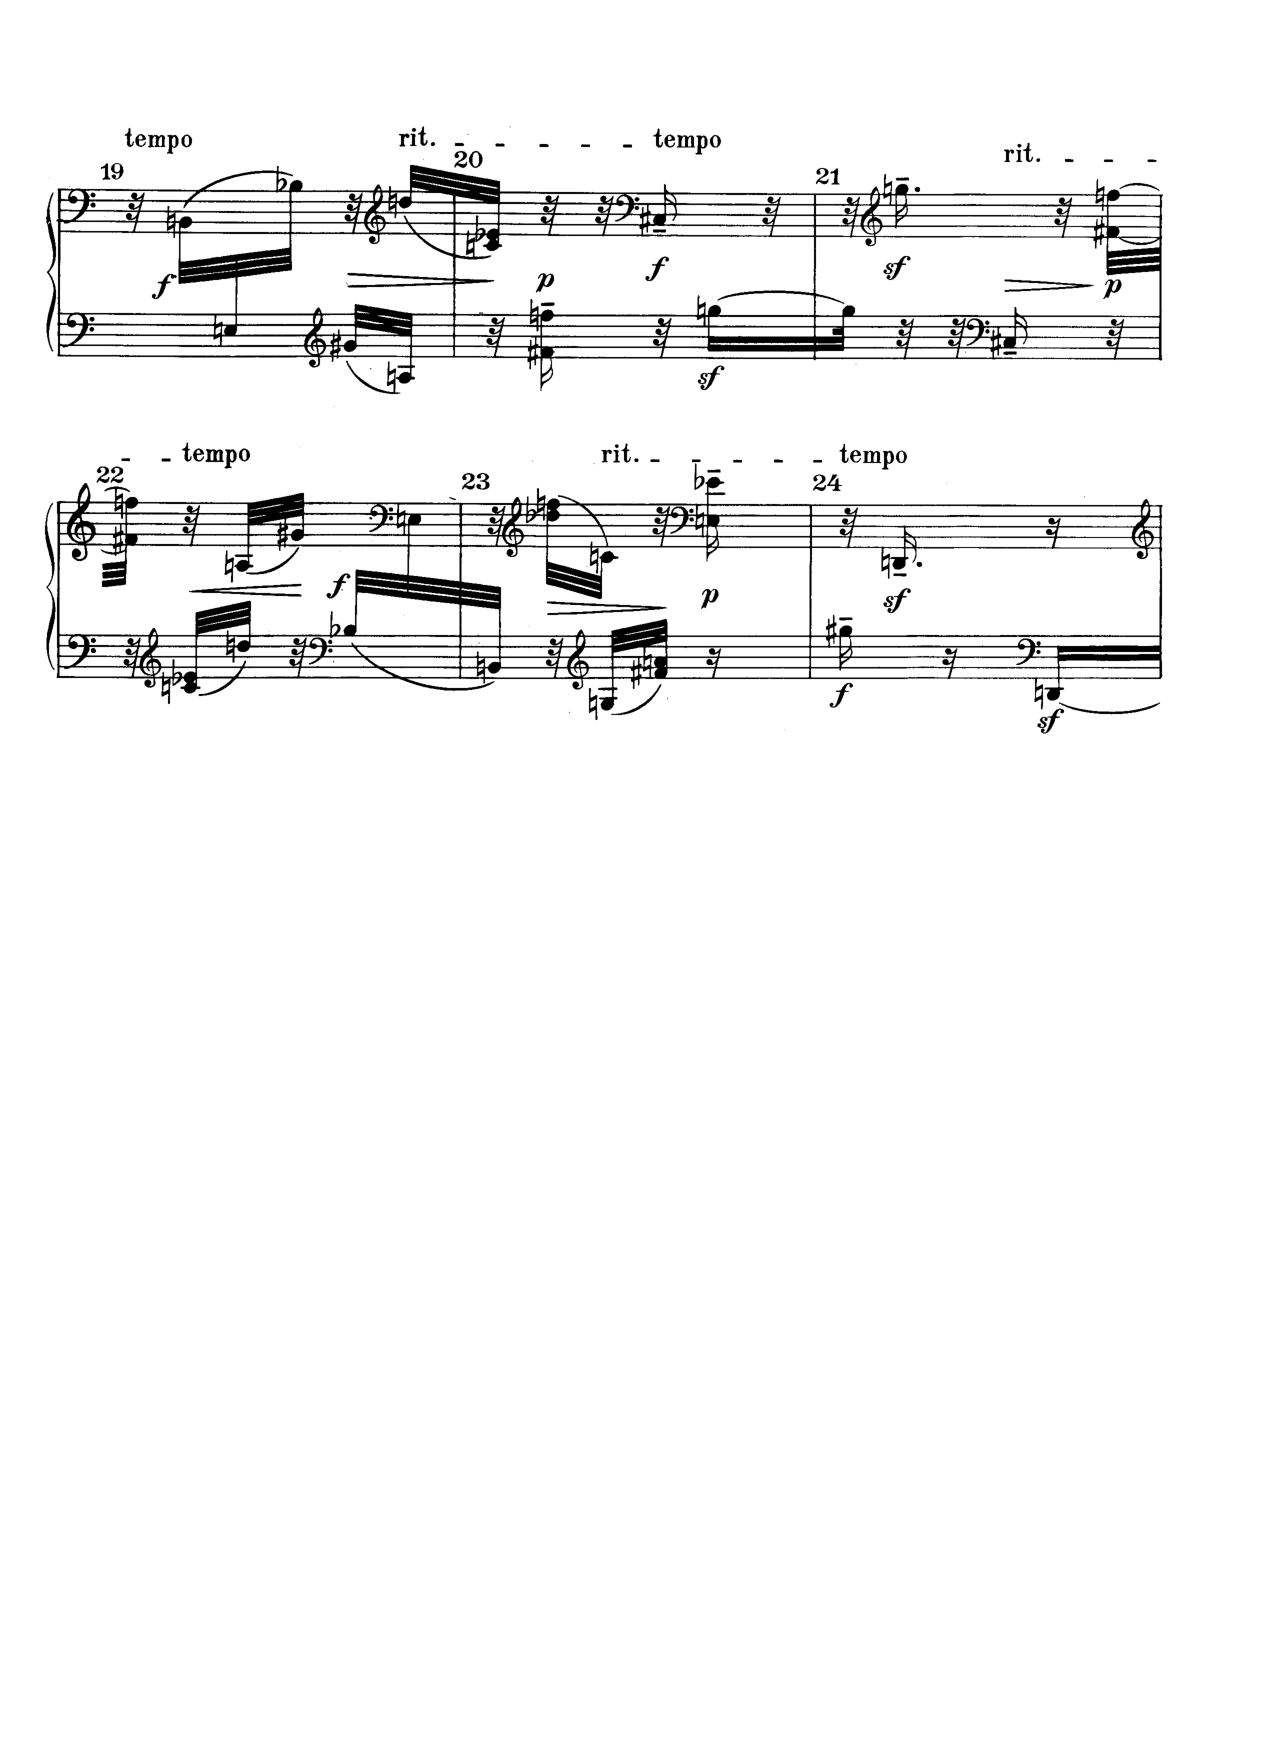
\includegraphics[width=6.5in]{figures/webern3.pdf}
		\caption[Bars 19--23 in Webern's Op.~27]{Bars 19--23 in Webern's Op.~27.}
    	\label{fig:webern-27-c}
	\end{figure}

	\begin{figure}[htbp]
    	\centering
		\begin{tikzcd}
	    	& [-1em] & [-1em] & [-1em] E\flat \arrow[dr] & [-1em] & [-1em] & [-1em] B\flat \arrow[dr] & [-1em] & [-1em] & [-1em] \\
	    	E \arrow[r] & [-1em] F \arrow[r] & [-1em] C\sharp \arrow[ur] \arrow[dr] & [-1em] & [-1em] D \arrow[r] & [-1em] G\sharp \arrow[ur] \arrow[dr] & [-1em] & [-1em] F\sharp \arrow[r] & [-1em] G \arrow[r] & [-1em] B \\
	    	& [-1em] & [-1em] & [-1em] C \arrow[ur] & [-1em] & [-1em] & [-1em] A \arrow[ur] & [-1em] & [-1em] & [-1em]
    	\end{tikzcd}
		\caption[An Aggregate Realization of Bars 19--23 in Webern's Op.~27]{The underlying partial order depicted in this aggregate realization is denoted by $D_3$.}
    	\label{fig:webern-aggregate-d}
	\end{figure}

	\noindent The last step in figuring out Webern's total order, according to the theoretical assumptions made so far, is to take intersections of the partial orders depicted above with aggregate realizations. Assuming the presentation of the series could actually be heard despite the numerous pitfalls represented by all the registral displacements in the piece, and furthermore assuming twelve ordered and different pitch classes could be freely inverted and transposed by ear almost instantly, the intersection $D_1 \cap D_2$ at measure 10 would possibly be inferred. An aggregate realization of the intersection is shown in Fig.~\ref{fig:webern-aggregate-e}. However, since there would still be three incomparabilities that preventing full comprehension the underlying series.

	\begin{figure}[htbp]
    	\centering
		\begin{tikzcd}
	    	& [-1em] E \arrow[dr] & [-1em] & [-1em] & [-1em] D \arrow[dr] & [-1em] & [-1em] & [-1em] & [-1em] G \arrow[dr] & [-1em] \\
	    	* \arrow[ur] \arrow[dr] & [-1em] & [-1em] C\sharp \arrow[r] & [-1em] E\flat \arrow[ur] \arrow[dr] & [-1em] & [-1em] G\sharp \arrow[r] & [-1em] A \arrow[r] & [-1em] B\flat \arrow[ur] \arrow[dr] & [-1em] & [-1em] B \\
	    	& [-1em] F \arrow[ur] & [-1em] & [-1em] & [-1em] C \arrow[ur] & [-1em] & [-1em] & [-1em] & [-1em] F\sharp \arrow[ur] & [-1em] \\
    	\end{tikzcd}
		\caption[Intersecting Bars 1--7 with Bars 8--10 in Webern's Op.~27]{The intersection $D_1 \cup D_2$.}
    	\label{fig:webern-aggregate-e}
	\end{figure}

	\noindent The next two pictures depict aggregate realizations for the intersections $D_1 \cap D_3$ and $D_2 \cap D_3$. Having reached measure 23, Webern's series can finally be obtained. Both intersections, however, still carry incomparabilities, so taking the intersection of all three aggregate realizations is still necessary.

	\begin{figure}[htbp]
    	\centering
		\begin{tikzcd}
	    	& [-1em] & [-1em] & [-1em] & [-1em] & [-1em] & [-1em] & [-1em] B\flat \arrow[dr] & [-1em] & [-1em] & [-1em] \\
	    	E \arrow[r] & [-1em] F \arrow[r] & [-1em] C\sharp \arrow[r] & [-1em] E\flat \arrow[r] & [-1em] C \arrow[r] & [-1em] D \arrow[r] & [-1em] G\sharp \arrow[ur] \arrow[dr] & [-1em] & [-1em] F\sharp \arrow[r] & [-1em] G \arrow[r] & [-1em] B \\
	    	& [-1em] & [-1em] & [-1em] & [-1em] & [-1em] & [-1em] & [-1em] A \arrow[ur] & [-1em] & [-1em] & [-1em]
    	\end{tikzcd}
		\caption[Intersecting Bars 1--7 with Bars 19--23 in Webern's Op.~27]{The intersection $D_1 \cup D_3$.}
    	\label{fig:webern-aggregate-f}
	\end{figure}

	\begin{figure}[htbp]
    	\centering
		\begin{tikzcd}
	    	& [-1em] & [-1em] & [-1em] E\flat \arrow[dr] & [-1em] & [-1em] & [-1em] & [-1em] & [-1em] & [-1em] & [-1em] \\
	    	E \arrow[r] & [-1em] F \arrow[r] & [-1em] C\sharp \arrow[ur] \arrow[dr] && [-1em] D \arrow[r] & [-1em] G\sharp \arrow[r] & [-1em] A \arrow[r] & [-1em] B\flat \arrow[r] & [-1em] F\sharp \arrow[r] & [-1em] G \arrow[r] & [-1em] B \\
	    	& [-1em] & [-1em] & [-1em] C \arrow[ur] & [-1em] & [-1em] & [-1em] & [-1em] & [-1em] & [-1em] & [-1em]
    	\end{tikzcd}
		\caption[Intersecting Bars 8--10 with Bars 19--23 in Webern's Op.~27]{The intersection $D_2 \cup D_3$.}
    	\label{fig:webern-aggregate-g}
	\end{figure}

	\begin{figure}[htbp]
    	\centering
		\begin{tikzcd}
	    	E \arrow[r] & [-1em] F \arrow[r] & [-1em] C\sharp \arrow[r] & [-1em] E\flat \arrow[r] & [-1em] C \arrow[r] & [-1em] D \arrow[r] & [-1em] G\sharp \arrow[r] & [-1em] A \arrow[r] & [-1em] B\flat \arrow[r] & [-1em] F\sharp \arrow[r] & [-1em] G \arrow[r] & [-1em] B
    	\end{tikzcd}
		\caption[The intersection of Bars 1--7, 8--10, and 19--23 in Webern's Op.~27]{The intersection $D_1 \cup D_2 \cup D_3$.}
    	\label{fig:webern-aggregate-h}
	\end{figure}
\end{example}

There is much to be said about Ex.~\ref{starr-webern-example}, particularly in what regards the aural perception of the composer's constructs. There is even more to be said when taking into consideration the fact that, as the twentieth-century unraveled, it became in many cases increasingly more difficult to establish how a piece of music was constructed with the presence of the score alone, much less simply by aural inference. It becomes less straightforward to determine the role of the listener in these cases, especially whenever one insists that the listener should be able to aurally infer \emph{every} construct in a musical composition. It can be argued that, as composers differentiate themselves from common practice, compositional technique becomes more subjective, and often indiscernible in the musical discourse. That does not mean, however, that musical fruition should be hindered in any sense, or that the composer's channel of communication with the listener has been narrowed in any way. It is simply the case that, even when not every single part of a structure is fathomed, the structure itself can still be experienced.

%We do not need a blueprint to live in a house, we do not need a wrench to drive a car, and we certainly do not begin to understand the intricacies of the very universe in which we exist. And we do exist nonetheless.

The role of the analyst, on the other hand, also becomes more difficult to define. Whenever the structure of a piece of music becomes impossible to follow from its score alone, a theorist must reconsider the weight of musicological work in the analysis of such repertoire. In other words, it may very well be impossible to analyze a composition without resorting to the composer, or to a musicological study thereof. That is especially the case with algorithmic composition, which is a major avenue to which we shall apply our main object of study. Analyzing an algorithmically generated piece of music without prior knowledge of the algorithm itself can only go as far as devising hearing strategies for the piece, as well as conjecturing what the algorithm might have been. It may be of substantial value, it may even carry more value than an analysis of the algorithm itself. And, just like with any piece of software, understanding the code is not a prerequisite to using said software, much less to determining whether it fulfills its purpose, or whether it is a good piece of software or not. However, if one intends to determine precisely how a piece of music was \emph{constructed}, then knowledge of its blueprint becomes essential. And that determination is often of primary interest to composers.

The compositional techniques we are about to define and generalize in this study are notoriously of structural relevance. It does not mean that they cannot be aurally discerned, and in fact many authors devote considerable time devising hearing strategies for them, particularly when they are used to structure pitch. Nevertheless, our approach here will be restricted to the intrinsic qualities of these techniques, and we shall not pursue their aural perception in depth, simply because there may not be any intention from the composer's part for them to be heard at all. A familiar example might be the music of Stravinsky. Upon analyzing his use of rotational arrays, it becomes clear that the composer uses them as a generative techniques, rather than as a foreground musical entities. Analyzing such pieces often resort to techniques that have no connection whatsoever to any sort of hearing strategy, like Forte's employment of K and Kh set complexes, which yield a nexus set that ultimately cannot be heard. We aggravate this discussion with the idea that, more often than not, we shall employ the techniques we are about to present to dimensions other than pitch, and in particular to algorithmically determining spectral components and timbre. In this sense, their outcomes become textural elements of a composition, but still well within the canon of tasks a composer needs to exercise in the craft of a piece.

%\clearpage
%\thispagestyle{plain}
%\begin{landscape}
%\begin{figure}
%\begin{center}
%\includegraphics[width=6in]{images/LaTeX2e_logo.eps}
%\caption{\LaTeX 2\ensuremath{\epsilon.} logo}\label{biglogo}
%\end{center}
%\end{figure}
%\end{landscape}

%\begin{table}[htbp]
%\caption{A sample Table}\label{first}
%\begin{tabularx}{6.5in}{XXX}
%\hline
%First & Second & Third \\
%\hline
%12 & 45 & 26 \\
%17 & 32 & 93 \\
%text & 51 & can be there too. \\
%\hline
%\end{tabularx}
%\end{table}

%\begin{table}
%\caption{Feasible triples for highly variable Grid}
%\label{tbl1}
%\begin{tabularx}{6.5 in}{r l X}
%\hline {{Time (s)}} & {{Triple chosen}} & {{Other feasible triples}} \\ \hline
%0 & (1, 11, 13725) & (1, 12, 10980), (1, 13, 8235), (2, 2, 0), (3, 1, 0) \\
%2745 & (1, 12, 10980) & (1, 13, 8235), (2, 2, 0), (2, 3, 0), (3, 1, 0) \\
%5490 & (1, 12, 13725) & (2, 2, 2745), (2, 3, 0), (3, 1, 0) \\
%\hline
%\end{tabularx}
%\end{table}

%\begin{table}[h!t!]
%\begin{tabularx}{6.5 in}{r l X}
%\multicolumn{3}{l}{Table \ref{tbl1}. Continued}\\%
%\hline {{Time (s)}} & {{Triple chosen}} & {{Other feasible triples}} \\ \hline
%115290 & (1, 13, 16470) & (2, 2, 2745), (2, 3, 0), (3, 1, 0) \\
%118035 & (1, 13, 13725) & (2, 2, 2745), (2, 3, 0), (3, 1, 0) \\
%120780 & (1, 13, 16470) & (2, 2, 2745), (2, 3, 0), (3, 1, 0) \\
%123525 & (1, 13, 13725) & (2, 2, 2745), (2, 3, 0), (3, 1, 0) \\
%\hline
%\end{tabularx}
%\end{table}
